\documentclass[11pt]{article}
\usepackage{fullpage}
\usepackage{graphicx}
\usepackage{url}
\usepackage{clrscode}
\usepackage{amsmath}
\usepackage{amssymb}
% \usepackage{algorithm}
% \usepackage{algpseudocode}

\setlength{\parindent}{0pt}
\setlength{\parskip}{8pt}

\title{CS140 - Assignment 8\\\small{Due: Sunday,  Mar. 31st at 11:59pm}}
\author{}
\date{}

\begin{document}

\maketitle

\begin{center}
% \includegraphics[scale=0.5]{figures/dfs.jpg}
{\footnotesize http://xkcd.com/761/}
\end{center}

Notes: 
\begin{itemize}
\item Many of the algorithms below can be accomplished by either modifying the graph and applying a known algorithm or slightly modifying a known algorithm.  Try thinking of these \emph{first} as they will save you a lot of work, and writing :)  I don't expect long answers, but be precise.
\item You will be graded on efficiency!
\item If not specified in the problem, you may assume whatever graph representation makes your algorithm more efficient (adjacency list or adjacency matrix).  State which one you are using.
\end{itemize}

\begin{enumerate}
	
\item \textbf{[8 points]} State whether the following statements about a graph $G$ that is undirected and connected are true or false and justify your answer.

\begin{enumerate}

\item Prim's algorithm works correctly if $G$ has negative edge weights.

    \textbf{Answer}: True.  Because Prim's algorithm seeks minimum edges, and negative numbers would still maintain the minimum's cut property.

\item The shortest path between two nodes is always part of some MST.
\begin{figure}[h]
    \centering
    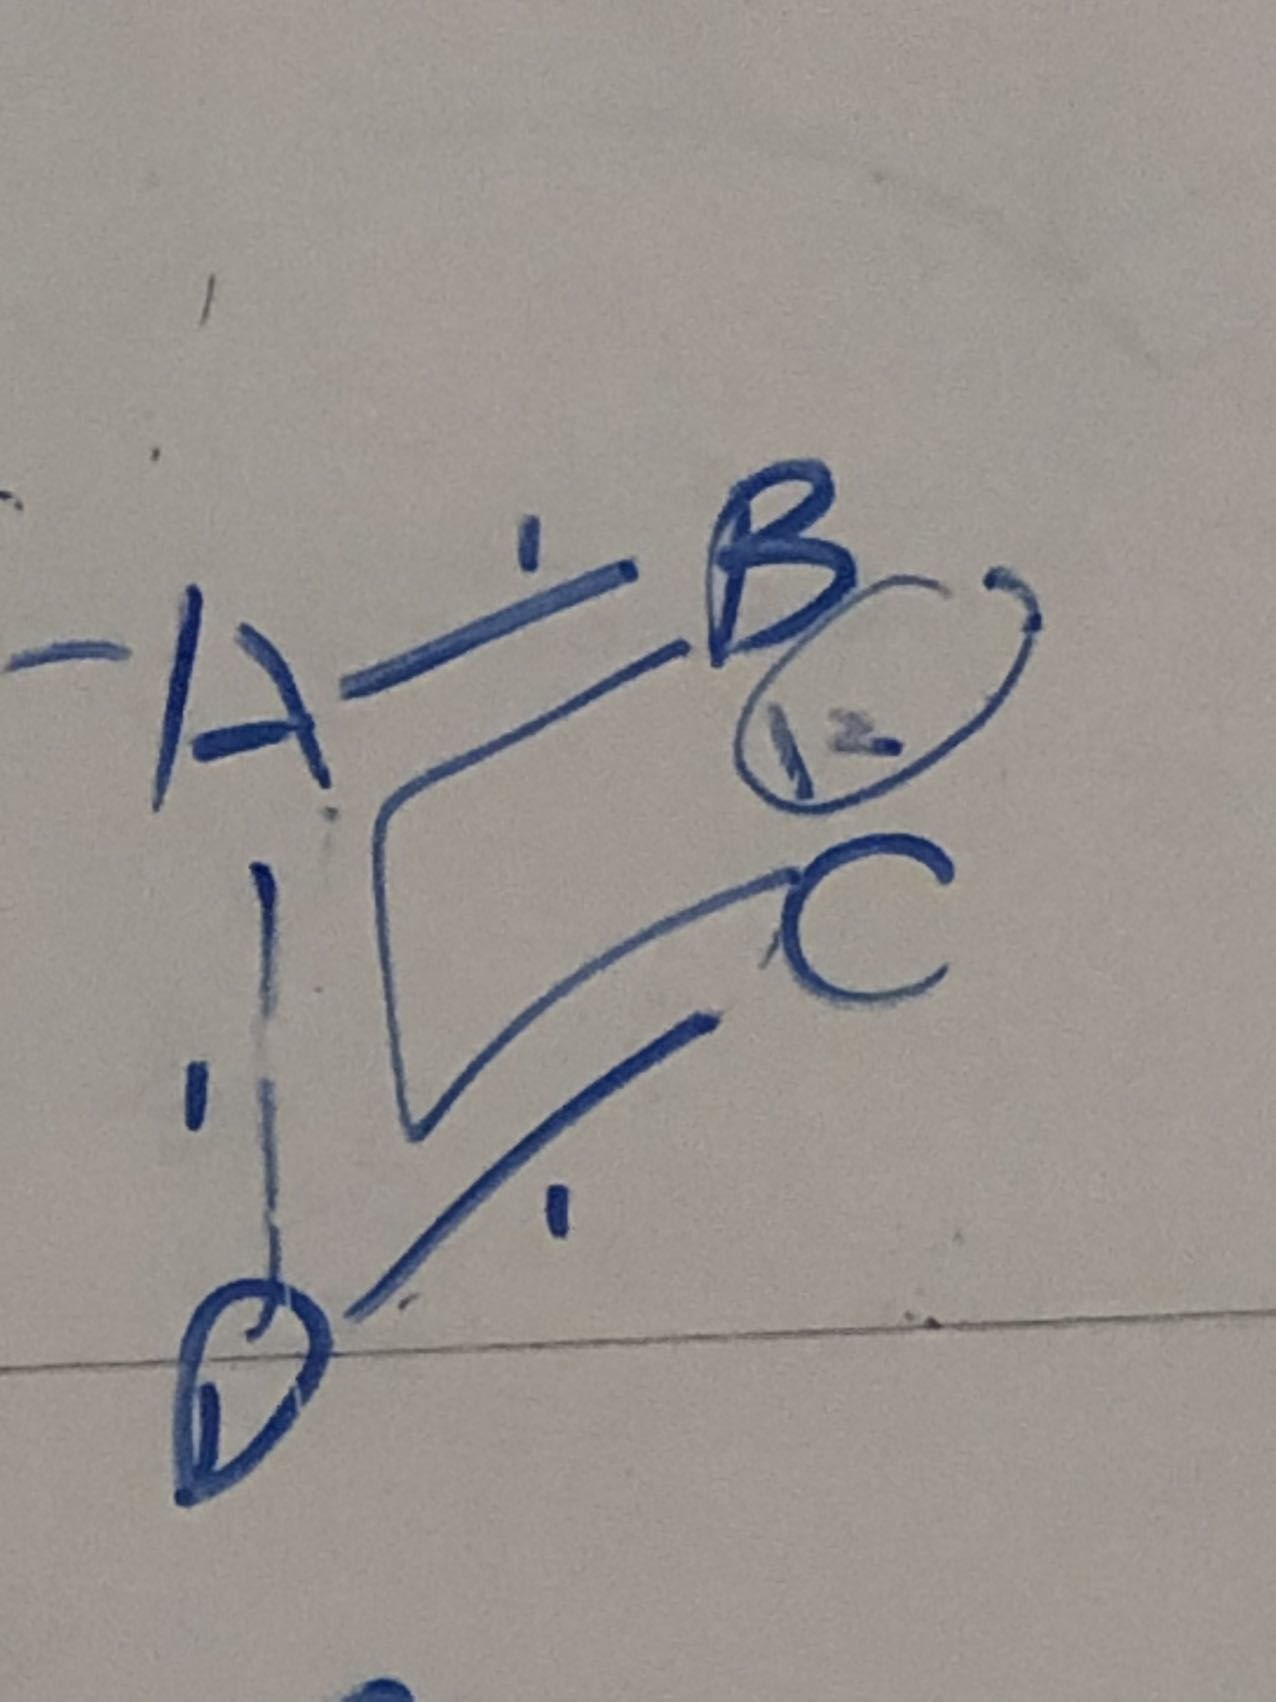
\includegraphics[width=0.3\linewidth]{WechatIMG308.jpeg}
    \caption{Enter Caption}
    \label{fig:enter-label}
\end{figure}
\textbf{Answer}: False. Because  the shortest path from B to C is 2 but MST is $B=>A=>D=>C$, which does not include path $BC$.


\end{enumerate}
\item \textbf{[5 points]} Write pseudocode for an algorithm which, given an undirected graph $G$ and a particular edge $e$ in it, determines whether $G$ has a cycle containing $e$.  What is the runtime of this algorithm?

\emph{Thoughts}: The core concept involves taking the edge $e$ defined by the vertices $u$ and $v$, and considering whether there's an alternate route connecting $u$ to $v$ after removing $e$ from the graph. If such a path exists, then a cycle is present and $e$ forms part of that cycle. If no such path exists, then the edge $e$ is critical for the connection between $u$ and $v$, indicating the absence of a cycle containing $e$. For the task of determining whether there's a path from $u$ to $v$, you can use DFS or BFS. We choose to use DFS.

\begin{codebox}
\Procname{$\proc{ModifiedDFS}(G, curr, end, visited):$}
    \li \If $curr = end$
    \li     \Return $True$
        \End
    \li $visited[curr] \gets True$
    \li \For each $adjacent$ vertex $v$ of $curr$
    \li   \hspace{4 pt}  \If not $visited[v]$ \textbf{and} $\proc{ModifiedDFS}(G, v, end, visited)$ 
    \li         \hspace{12 pt} \Return $True$
            \End
        \End
    \li \Return $False$
\end{codebox}

\begin{codebox}
\Procname{$\proc{HasCycle}(G, e):$}
\li $(start, end) \gets e$
\li $GWithoutE \gets G.\proc{Remove}(e)$
\li $visited \gets \{False \times \proc{Length}(V)\}$
\li \Return $\proc{ModifiedDFS}(GWithoutE, start, end, visited)$
\end{codebox}
The \textbf{runtime} is the same as that of DFS - $O(V+E)$.

\item \textbf{[8 points]} Often there are multiple shortest paths between nodes of a graph.  Write pseudocode for an algorithm that given an undirected, unweighted graph $G$ and nodes $u,v \in V$, outputs the number of distinct shortest paths from $u$ to $v$.  What is the running time?

\emph{Thoughts}: You have your start node, u, and your end node, v. The gist is that you need to define 2 global variables which will be arrays which will record data for each node. Call the first array, d (for distance) which records the distance from the start node u to that particular vertex or node. d will be initialized to infinity except the d-position corresponding to the start node, whose value is 0, since it takes 0 units of distance to reach the start node from itself. And the second array, c (for count), which will record the count of the number of shortest paths from the start node (u) thus far. 

Essentially we use BFS to traverse our node but with a few, 2, modifications.
The first modification is that if the distance from the current node plus one is equal to the distance to the next node (from the start node), then we know that there is another path we can get to that particular node from the start node and so we increment the c-position-value of the next node after the current one as so:
if dist[current] + 1 == dist[next]:
	count[next] += count[current]

The second modification is that if the distance to the next node is greater than the distance to the current node (from the start node) + 1, then we know we have identified a new shortest path so we update the c-array-position of the next node to be that of the current node. As so:
if d[next] $>$ d[curr] + 1:
	count[target] = count[current]

\begin{codebox}
\Procname{$\proc{distinctShortestPaths}(G, u, v):$}
\li \For each vertex $x \in V(G)$
\li     \hspace{12 pt} $dist[x] \leftarrow \infty$
\li     \hspace{12 pt} $count[x] \leftarrow 0$
\li $dist[u] \leftarrow 0$
\li $count[u] \leftarrow 1$
\li $\proc{Enqueue}(Q, u)$
\li \While !$\proc{Empty}(Q)$
\li     \hspace{12 pt} $current \leftarrow \proc{Dequeue}(Q)$
\li     \hspace{12 pt} \For each adjacent vertex $next$ of $current$
\li     \hspace{30 pt}\If $dist[next] = \infty$
\li             \hspace{42 pt} $dist[next] \leftarrow dist[current] + 1$
\li                 \hspace{42 pt} $count[next] \leftarrow count[current]$
\li                 \hspace{42 pt} $\proc{Enqueue}(Q, next)$
\li     \hspace{30 pt} \ElseIf $dist[next] = dist[current] + 1$
\li      \hspace{42 pt}        $count[next] \leftarrow count[next] + count[current]$ 
\li \ElseIf $dist[next] > dist[current] + 1$
\li       \hspace{42 pt}                $count[next] \leftarrow count[current]$ \End \End \End
\li \Return $count[v]$
\end{codebox}

The running time is $O(V+E)$ as for BFS.




\item \textbf{[5 points]} Given a directed graph $G = (V,E)$ with positive edge weights and a particular node $v_i \in V$, give an efficient algorithm for finding the shortest paths between \textbf{all pairs of nodes}, with the one restriction that these paths must all pass through $v_i$.  Give the runtime of your algorithm.  Points will be deducted for an inefficient algorithm.

\emph{Hints:}  \begin{itemize}

\item[-] Any path in this problem can be seen as two parts, the part to $v_i$ and the part from $v_i$.
\item[-] Look at how we determined if a graph was strongly connected.

\begin{enumerate}
Dijkstra's Algorithm finds the shortest path between a given node and all other nodes in a graph. So we run Dijkstra's algorithm from the node  $v_i $ to every other node in V to get the shortest path from  $v_i $  to all other nodes. Then we run Dijkstra's algorithm on the same graph but with a reversed direction of every edge again  starting from $v_i $. This way it created the shortest paths for all pairs of nodes. Then we combine these two path. So if we want go from a to b,the shortest path would be a to  $v_i $  and  $v_i $  to b. The runtime for just  Dijkstra's algorithm using Fib heap as a priority queue is $O(|V| log |V| + |E|)$  if we run two times it should times two but at the end$ O(|V| log |V| + |E|) $stays the same since it dominates. 

\end{enumerate}


\end{itemize}

\item \textbf{[5 points]} If a graph does not have a negative cycle, when calculating the shortest paths from a given vertex using the Bellman-Ford algorithm, we can stop early and do not need to do all $|V|-1$ iterations and will still have a correct answer for all the shortest paths from that vertex.  Describe how to modify the Bellman-Ford algorithm to stop early when all of the distances are already correct.

For Bellman-Ford algorithm, we listed all the vertex in a table(lets say there's n vertexes) and marked the distance to every vertex to infinity,  and set the starting vertex distance to zero. We initialize a boolean values to keep track if each element is updated or not, and set it as false at the start of each iteration. Then we go through the graph for first iteration using a loop (meaning from the first vertex to the last vertex). Within the first iteration, we go from the starting index to the next vertexes it could reach, and we mark the distance in the table. Then we move to the second vertex and see which vertex we could reach directly, and mark the distance if it's smaller than the previous distance, if we changed it, we update the boolean variable to true.  We repeat this steps for iterations( for start of  each iteration the variable is reset to false). At the end of each iteration, we check if the variable is false, if it's false we which means that no shorter paths were found, then we stop the algorithms.



\item \textbf{[6 points]} Given an undirected graph $G$ with nonnegative edge weights $w_e \ge 0$.  Suppose you have calculated the minimum spanning tree of $G$ and also the shortest paths to all nodes from a particular node $s \in V$.  Now, suppose that each edge weight is increased by 1, i.e. the new weights are $w'_e = w_e + 1$.

	\begin{enumerate}

	\item (3 points) Does the minimum spanning tree change?  Give an example where it does or prove that it cannot change.
It does not change because for minimum spanning tree it basically is trying to find the next edge with smallest value to connect until all vertexes are connected with no cycle in it. Therefore, if all the edges add one, the order would still remain the same. Lets say we have 2, 3, 4 as value for three edges which form a triangle as a graph. The MST would be connecting 2 and 3. After we add 1 to each graph, we have 3,4,5. And the MST would still be the same except the value of edge is 3,4 now. This is because Prim's algorithm seeks minimum edges, and after adding 1 to each number, they would still maintain the minimum's cut property.

	\item (3 points) Do the shortest paths from $s$ change?  Given an example where it does or prove that it cannot change.
Yes. Imagine a quadrilateral whose vertexes labeled the as abcd. Lable ab is 1, ac is 1, cd is 1, and bd is  4. The shortest path from B to D right now is 3 which is bacd.  If we add 1 to each edge, ab is 2, ac is 2, cd is 2, and bd is  5. Now the shortest path from B to D would be 5 which is bd since bacd is 6 now.
a —1— b
| 1        |4
c— 1—d



	\end{enumerate}

\end{enumerate}

\end{document}
